\subsection{蛇形图}

命题 1. --- 考虑一个 A-模的交换图

\[
\begin{array}{c} \mathrm{M} \xrightarrow {u} \mathrm{N} \xrightarrow {v} \mathrm{P} \\ f \Big \downarrow \qquad \qquad \qquad g \Big \downarrow \qquad \qquad \qquad h \Big \downarrow \\ \mathrm{M} ^ {\prime} \xrightarrow {u ^ {\prime}} \mathrm{N} ^ {\prime} \xrightarrow {v ^ {\prime}} \mathrm{P} ^ {\prime}. \end{array}\tag{4}
\]

假设 (4) 的两行是正合的。则：

\begin{enumerate}
\def\labelenumi{(\roman{enumi})}
\tightlist
\item
  若 h 是单射，我们有
\end{enumerate}

\[
\operatorname{Im} (g) \cap \operatorname{Im} \left(u ^ {\prime}\right) = \operatorname{Im} \left(u ^ {\prime} \circ f\right) = \operatorname{Im} (g \circ u).\tag{5}
\]

\begin{enumerate}
\def\labelenumi{(\roman{enumi})}
\setcounter{enumi}{1}
\tightlist
\item
  若 f 是满射，我们有
\end{enumerate}

\[
\operatorname{Ker} (g) + \operatorname{Im} (u) = \operatorname{Ker} \left(v ^ {\prime} \circ g\right) = \operatorname{Ker} (h \circ v).\tag{6}
\]

让我们证明 (i)。显然我们有

\[
\operatorname{Im} \left(u ^ {\prime} \circ f\right) = \operatorname{Im} (g \circ u) \subset \operatorname{Im} (g) \cap \operatorname{Im} \left(u ^ {\prime}\right).
\]

反之，设 \(y' \in \operatorname{Im}(g) \cap \operatorname{Im}(u')\) 。存在 \(y \in \mathbf{N}\) 使得 \(y' = g(y)\) 。由于 \(v' \circ u' = 0\) ，我们有 \(0 = v'(y') = v'(g(y)) = h(v(y))\) ，从而 \(v(y) = 0\) ，因为 \(h\) 是单射。由于 \((u, v)\) 是正合序列，存在 \(x \in \mathbf{M}\) 使得 \(y = u(x)\) ，从而 \(y' = g(u(x))\) .

让我们证明 (ii)。由于 \(v \circ u = 0\) 且 \(v' \circ u' = 0\) ，显然

\[
\operatorname{Ker} (g) + \operatorname{Im} (u) \subset \operatorname{Ker} \left(v ^ {\prime} \circ g\right) = \operatorname{Ker} (h \circ v).
\]

反之，设 \(y \in \operatorname{Ker}(v' \circ g)\) 。然后 \(g(y) \in \operatorname{Ker}(v')\) ，并且存在 \(x' \in M'\) 使得 \(u'(x') = g(y)\) 由于序列 \((u', v')\) 是正合的。由于 \(f\) 是满射的，存在 \(x \in M\) 使得 \(f(x) = x'\) ，从而 \(g(y) = u'(f(x)) = g(u(x))\) ；由此我们得出结论 \(y - u(x) \in \operatorname{Ker}(g)\) ，这就完成了证明。

引理1. —— 考虑一个A-模的交换图

\[
\begin{array}{c} \mathbf {M} \xrightarrow {\quad u \quad} \mathbf {N} \\ f \Big \downarrow \qquad \qquad \qquad \qquad \qquad \qquad \qquad \qquad g \Big \downarrow \\ \mathbf {M} ^ {\prime} \xrightarrow {\quad u ^ {\prime} \quad} \mathbf {N} ^ {\prime}. \end{array}\tag{7}
\]

那么存在唯一的同态 \(u_1: \text{Ker}(f) \to \text{Ker}(g)\) 和唯一的同态 \(u_2: \text{Coker}(f) \to \text{Coker}(g)\) ，使得以下图表

\[
\begin{array}{c} \operatorname{Ker} (f) \xrightarrow {u _ {1}} \operatorname{Ker} (g) \\ i \Biggl \downarrow \\ \mathrm{M} \xrightarrow [ u ]{} \mathrm{N} \end{array}\tag{8}
\]

和

\begin{enumerate}
\def\labelenumi{(\arabic{enumi})}
\setcounter{enumi}{8}
\tightlist
\item
\end{enumerate}

\pandocbounded{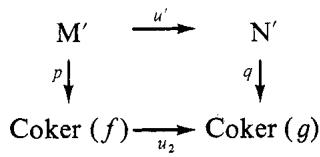
\includegraphics[keepaspectratio]{images/part001_11db974a.jpg}}

设它们是交换的，其中i和j表示典范单射，p和q表示典范满射。

事实上，若 \(x \in \operatorname{Ker}(f)\) ，我们有 \(f(x) = 0\) 和 \(g(u(x)) = u'(f(x)) = 0\) ，因此 \(u(x) \in \operatorname{Ker}(g)\) ，于是 \(u_1\) 的存在性与唯一性立即得出。同样地，我们有

\[
u ^ {\prime} (f (\mathbf {M})) = g (u (\mathbf {M})) \subset g (\mathbf {N}),
\]

因此 \(u'\) 通过取商给出一个同态

\[
u _ {2}: \operatorname{Coker} (f) \rightarrow \operatorname{Coker} (g),
\]

这是使（9）可交换的唯一同态。

现在从A-模的交换图（4）出发；根据引理1，它对应一个交换图

\[
\begin{array}{c c c c c} \operatorname{Ker} (f) \xrightarrow {u _ {1}} & \operatorname{Ker} (g) \xrightarrow {v _ {1}} & \operatorname{Ker} (h) \\ i \Big \downarrow & j \Big \downarrow & k \Big \downarrow \\ \mathbf {M} & u & \mathbf {N} & v & \mathbf {P} \\ f \Big \downarrow & g \Big \downarrow & h \Big \downarrow \\ \mathbf {M} ^ {\prime} & u ^ {\prime} & \mathbf {N} ^ {\prime} & v ^ {\prime} & \mathbf {P} ^ {\prime} \\ p \Big \downarrow & q \Big \downarrow & r \Big \downarrow \\ \operatorname{Coker} (f) \xrightarrow {u _ {2}} & \operatorname{Coker} (g) \xrightarrow {v _ {2}} & \operatorname{Coker} (h) \end{array}\tag{10}
\]

其中 \(i, j, k\) 是典范单射， \(p, q, r\) 是典范满射， \(u_{1}, u_{2}\) （相应地， \(v_{1}, v_{2}\) ）是由 \(u\) , \(u'\) （相应地， \(v, v'\) ）依引理1得出的同态。

命题2. --- 假设在交换图 (4) 中，序列 \((u, v)\) 与 \((u', v')\) 是正合的。则：

\begin{enumerate}
\def\labelenumi{(\roman{enumi})}
\item
  我们有 \(v_{1} \circ u_{1} = 0\) ；若 \(u'\) 是单射的，则序列 \((u_{1}, v_{1})\) 是正合的。
\item
  我们有 \(v_2 \circ u_2 = 0\) ；若v是满射，则序列 \((u_2, v_2)\) 是正合的。
\item
  假设 \(u'\) 是单射且 \(v\) 是满射。则存在且仅存在一个同态 \(d: \operatorname{Ker}(h) \to \operatorname{Coker}(f)\) 具有以下性质：如果 \(z \in \operatorname{Ker}(h)\) , \(y \in \mathbf{N}\) 与 \(x' \in \mathbf{M}'\) 满足关系 \(v(y) = k(z)\) 和 \(u'(x') = g(y)\) ，我们有 \(d(z) = p(x')\) 。此外，序列
\end{enumerate}

(*) \(\operatorname{Ker}(f) \xrightarrow{u_1} \operatorname{Ker}(g) \xrightarrow{v_1} \operatorname{Ker}(h) \xrightarrow{d} \operatorname{Coker}(f) \xrightarrow{u_2} \operatorname{Coker}(g) \xrightarrow{v_2} \operatorname{Coker}(h)\) 是正合的。

\pandocbounded{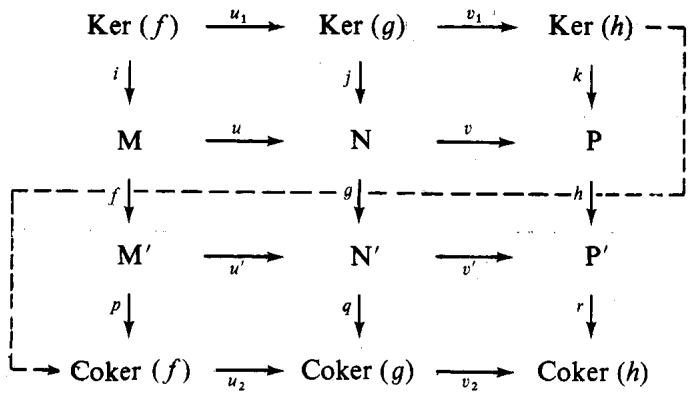
\includegraphics[keepaspectratio]{images/part001_0570902c.jpg}}

让我们证明 (i)。因为 \(u_{1}\) 与 \(v_{1}\) 分别同 \(u\) 和 \(v\) 到 \(\operatorname{Ker}(f)\) 与 \(\operatorname{Ker}(g)\) 上的限制具有相同的图像，我们有 \(v_{1} \circ u_{1} = 0\) 。我们有

\[
\operatorname{Ker} \left(v _ {1}\right) = \operatorname{Ker} (g) \cap \operatorname{Ker} (v) = \operatorname{Ker} (g) \cap \operatorname{Im} (u) = \operatorname{Im} (j) \cap \operatorname{Im} (u).
\]

但由命题1(i)，我们有 \(\operatorname{Ker}(v_1) = \operatorname{Im}(j \circ u_1) = \operatorname{Im}(u_1)\) 如果 \(u'\) 是单射。我们来证明 (ii)。由于 \(u_2\) 与 \(v_2\) 是由 \(u\) 和 \(v\) 通过取商得出的，显然 \(v_2 \circ u_2 = 0\) 。假设 \(v\) 是满射；由于 \(q\) 与 \(p\) 是满射，根据假设及命题 1 (ii)，我们有

\[
\begin{array}{r l} \operatorname{Ker} (v _ {2}) & = q (\operatorname{Ker} (v _ {2} \circ q)) = q (\operatorname{Ker} (v ^ {\prime}) + \operatorname{Im} (g)) = q (\operatorname{Ker} (v ^ {\prime})) \\ & = q (\operatorname{Im} (u ^ {\prime})) = \operatorname{Im} (q \circ u ^ {\prime}) = \operatorname{Im} (u _ {2} \circ p) = \operatorname{Im} (u _ {2}). \end{array}
\]

最后，我们来证明（iii）。对于 \(z \in \operatorname{Ker}(h)\) 存在 \(y \in \mathbf{N}\) 使得 \(v(y) = k(z)\) 因为 \(v\) 是满射；此外，我们有 \(v'(g(y)) = h(k(z)) = 0\) 因此存在唯一的 \(x' \in \mathbf{M}'\) 使得 \(u'(x') = g(y)\) 因为 \(u'\) 是单射。让我们证明元素 \(p(x') \in \operatorname{Coker}(f)\) 不依赖于元素 \(y \in \mathbf{N}\) ，只要它满足 \(v(y) = k(z)\) 。事实上，如果 \(y_1 \in \mathbf{N}\) 是另一个满足 \(v(y_1) = k(z)\) 的元素，我们有 \(y_1 = y + u(x)\) ，其中 \(x \in \mathbf{M}\) 。让我们证明，如果 \(x_1' \in \mathbf{M}'\) 满足 \(u'(x_1') = g(y_1)\) ，则 \(x_1' = x' + f(x)\) ；事实上，我们有 \(u'(x' + f(x)) = u'(x') + u'(f(x)) = g(y) + g(u(x)) = g(y + u(x)) = g(y_1)\) 最后，我们得出结论 \(p(x_1') = p(x') + p(f(x)) = p(x')\) 。因此我们可令 \(d(z) = p(x')\) ，并由此定义了一个映射 \(d: \operatorname{Ker}(h) \to \operatorname{Coker}(f)\) 。

如果现在 \(z_{1}, z_{2}\) 是 \(\operatorname{Ker}(h)\) 的元素，如果 \(\lambda_{1}, \lambda_{2} \in \mathbf{A}\) 和 \(z = \lambda_{1} z_{1} + \lambda_{2} z_{2}\) ，我们取元素 \(y_{1}\) 和 \(y_{2}\) 属于 \(\mathbf{N}\) ，使得 \(v(y_{1}) = k(z_{1})\) 和 \(v(y_{2}) = k(z_{2})\) ，并为 \(y \in \mathbf{N}\) 选取元素 \(\lambda_{1} y_{1} + \lambda_{2} y_{2}\) ；那么立即可以得出

\[
d (z) = \lambda_ {1} d (z _ {1}) + \lambda_ {2} d (z _ {2}),
\]

所以 d 是一个同态。

假设 \(z = v_1(t)\) 对于某个 \(t \in \operatorname{Ker}(g)\) ；我们将取 \(y \in \mathbf{N}\) 为元素 \(j(t)\) 。由于 \(g(j(t)) = 0\) ，我们得出结论 \(d(z) = 0\) ，因此 \(d \circ v_1 = 0\) 。反之，假设 \(d(z) = 0\) 。利用前面的记号，我们因此有 \(x' = f(x)\) ，其中 \(x \in M\) 。在这种情况下，我们有 \(g(y) = u'(f(x)) = g(u(x))\) ，或等价地 \(g(y - u(x)) = 0\) 。元素 \(y - u(x)\) 因此具有形式 \(j(n)\) 当 \(n \in \operatorname{Ker}(g)\) ，并且我们有

\[
k (z) = v (y) = v (u (x) + j (n)) = v (j (n)) = k \left(v _ {1} (n)\right);
\]

因为 \(k\) 是单射， \(z = v_{1}(n)\) ，这证明了序列(*)在 \(\operatorname{Ker}(h)\) 处是正合的。最后，我们仍有（使用相同的记号）

\[
u _ {2} (d (z)) = u _ {2} \left(p \left(x ^ {\prime}\right)\right) = q \left(u ^ {\prime} \left(x ^ {\prime}\right)\right) = q (g (y)) = 0 \quad \text {   hence   } \quad u _ {2} \circ d = 0.
\]

反之，假设一个元素 \(w = p(x')\) —— Coker \((f)\) 的元素 —— 满足

\[
u _ {2} (w) = u _ {2} \left(p \left(x ^ {\prime}\right)\right) = 0 \quad \left(\operatorname{with} x ^ {\prime} \in \mathbf {M} ^ {\prime}\right).
\]

我们因此有 \(q(u'(x')) = 0\) ，从而 \(u'(x') = g(y)\) 对于某个 \(y \in \mathbb{N}\) ；由于 \(v'(u'(x')) = 0\) ，我们有 \(v'(g(y)) = 0\) ，因此 \(h(v(y)) = 0\) ，换言之 \(v(y) = k(z)\) 对于某个 \(z \in \operatorname{Ker}(h)\) ，并且根据定义 \(w = d(z)\) ，这表明序列(*)在Coker( \(f\) )处是正合的。我们在(i)中看到它在Ker( \(g\) )处是正合的，在(ii)中看到它在Coker( \(g\) )处是正合的，这完成了(iii)的证明。

推论1. --- 假设图(4)是交换的且具有正合的行。则：

\begin{enumerate}
\def\labelenumi{(\roman{enumi})}
\item
  若 \(u'\) , \(f\) 和 \(h\) 是单射，则 \(g\) 是单射。
\item
  如果v、f和h是满射，则g是满射。
\end{enumerate}

断言 (i) 由命题 2 的断言 (i) 得出：事实上，我们有 \(\operatorname{Ker}(f) = 0\) 和 \(\operatorname{Ker}(h) = 0\) ，因此 \(\operatorname{Ker}(g) = 0\) 。

断言(ii)由命题2的断言(ii)得出：事实上，我们有Coker \(f\) = 0 且 Coker \(h\) = 0，因此 Coker \(g\) = 0.

推论 2. --- 假设图 (4) 是交换的且具有正合行。在这些条件下：

\begin{enumerate}
\def\labelenumi{(\roman{enumi})}
\item
  若g是单射，且f和v是满射，则h是单射。
\item
  若g是满射，且h与u'是单射，则f是满射。
\end{enumerate}

为了证明(i)，考虑该图表。

\[
\begin{array}{c c c c c} u (\mathbf {M}) & \xrightarrow {w} & \mathbf {N} & \xrightarrow {v} & \mathbf {P} \\ f ^ {\prime} \Big \downarrow & & g \Big \downarrow & & h \Big \downarrow \\ u ^ {\prime} (\mathbf {M} ^ {\prime}) & \xrightarrow {w ^ {\prime}} & \mathbf {N} ^ {\prime} & \xrightarrow {v ^ {\prime}} & \mathbf {P} ^ {\prime} \end{array}
\]

其中 \(f'\) 是与 \(g\) 到 \(u(\mathbf{M})\) 上的限制具有相同图像的映射， \(w\) 和 \(w'\) 为典范单射；显然该图表是交换的且行是正合的。此外 \(w'\) 是单射的，且根据假设 \(v\) 是满射；因此由命题2(iii)，我们有一个正合序列

\[
\operatorname{Ker} (g) \longrightarrow \operatorname{Ker} (h) \xrightarrow {d} \operatorname{Coker} \left(f ^ {\prime}\right);
\]

由于g是单射且 \(f'\) 是满射，因此我们有 Ker(h) = 0。

为证明(ii)，考虑如下图表。

\[
\begin{array}{c c c c c} \mathbf {M} & \stackrel {{u}} {{\longrightarrow}} & \mathbf {N} & \stackrel {{w}} {{\longrightarrow}} & v (\mathbf {N}) \\ f \Big \downarrow & & g \Big \downarrow & & h ^ {\prime} \Big \downarrow \\ \mathbf {M} ^ {\prime} & \stackrel {{u ^ {\prime}}} {{\longrightarrow}} & \mathbf {N} ^ {\prime} & \stackrel {{w ^ {\prime}}} {{\longrightarrow}} & v ^ {\prime} (\mathbf {N} ^ {\prime}) \end{array}
\]

此时 \(h'\) 是与 \(h\) 到 \(v(\mathbf{N})\) 上的限制具有相同图像的映射，且 \(w\) 和 \(w'\) 分别具有与 \(v\) 和 \(v'\) 相同的图像；此图表可交换且其行是正合的。此外 \(w\) 是满射，且根据假设 \(u'\) 是单射；因此由命题2(iii)，我们得到正合序列

\[
\operatorname{Ker} \left(h ^ {\prime}\right) \xrightarrow {d} \operatorname{Coker} (f) \longrightarrow \operatorname{Coker} (g);
\]

因为 \(g\) 是满射且 \(h'\) 是单射，因此我们有 Coker \((f) = 0\) 。

推论3（五引理）。——考虑一个A-模的交换图表

\[
\begin{array}{c c c c c c c c c} \mathbf {M} _ {1} & \xrightarrow {u _ {1}} & \mathbf {M} _ {2} & \xrightarrow {u _ {2}} & \mathbf {M} _ {3} & \xrightarrow {u _ {3}} & \mathbf {M} _ {4} & \xrightarrow {u _ {4}} & \mathbf {M} _ {5} \\ f _ {1} \Big \downarrow & & f _ {2} \Big \downarrow & & f _ {3} \Big \downarrow & & f _ {4} \Big \downarrow & & f _ {5} \Big \downarrow \\ \mathbf {M} _ {1} ^ {\prime} & \xrightarrow {u _ {1} ^ {\prime}} & \mathbf {M} _ {2} ^ {\prime} & \xrightarrow {u _ {2} ^ {\prime}} & \mathbf {M} _ {3} ^ {\prime} & \xrightarrow {u _ {3} ^ {\prime}} & \mathbf {M} _ {4} ^ {\prime} & \xrightarrow {u _ {4} ^ {\prime}} & \mathbf {M} _ {5} ^ {\prime} \end{array}
\]

其中的行是正合的。

\begin{enumerate}
\def\labelenumi{(\roman{enumi})}
\item
  若 \(f_{2}\) 和 \(f_{4}\) 是单射且 \(f_{1}\) 是满射，则 \(f_{3}\) 是单射。
\item
  若 \(f_{2}\) 和 \(f_{4}\) 都是满射且 \(f_{5}\) 是单射，则 \(f_{3}\) 是满射。
\end{enumerate}

特别地，如果 \(f_1, f_2, f_4\) 和 \(f_5\) 是同构，那么 \(f_3\) 也是。为证明 (i)，设 \(\tilde{\mathbf{M}}_2 = \text{Coker } (u_1), \tilde{\mathbf{M}}_2' = \text{Coker } (u_1')\) 并记 \(\tilde{f}_2: \tilde{\mathbf{M}}_2 \to \tilde{\mathbf{M}}_2'\) 由 \(f_2\) 推出的映射。由推论2(i)可知 \(\tilde{f}_2\) 是单射的。将推论1(i)应用于该图表

\[
\begin{array}{c c c c c} \tilde {\mathbf {M}} _ {2} & \xrightarrow {\tilde {u} _ {2}} & \mathbf {M} _ {3} & \xrightarrow {u _ {3}} & \mathbf {M} _ {4} \\ \tilde {f} _ {2} \Big \downarrow & & f _ {3} \Big \downarrow & & f _ {4} \Big \downarrow \\ \tilde {\mathbf {M}} _ {2} ^ {\prime} & \xrightarrow {\tilde {u} _ {2} ^ {\prime}} & \mathbf {M} _ {3} ^ {\prime} & \xrightarrow {u _ {3} ^ {\prime}} & \mathbf {M} _ {4} ^ {\prime} \end{array}
\]

其中 \(\tilde{u}_2\) 和 \(\tilde{u}_2'\) 是由 \(u_2\) 和 \(u_2'\) 得出的，我们看到 \(f_3\) 是单射。

为了证明(ii)，设 \(\tilde{\mathbf{M}}_{4} = \operatorname{Ker}(u_{4}), \tilde{\mathbf{M}}_{4}' = \operatorname{Ker}(u_{4}')\) 并记 \(\tilde{f}_{4}: \tilde{\mathbf{M}}_{4} \to \tilde{\mathbf{M}}_{4}'\) 由 \(f_{4}\) 诱导的映射。由推论2(ii)可知， \(\tilde{f}_{4}\) 是满射的。将推论1(ii)应用于该图表

\[
\begin{array}{c c c c c} \mathbf {M} _ {2} & \xrightarrow {u _ {2}} & \mathbf {M} _ {3} & \xrightarrow {\tilde {u} _ {3}} & \tilde {\mathbf {M}} _ {4} \\ f _ {2} \Big \downarrow & & f _ {3} \Big \downarrow & & \tilde {f} _ {4} \Big \downarrow \\ \mathbf {M} _ {2} ^ {\prime} & \xrightarrow {u _ {2} ^ {\prime}} & \mathbf {M} _ {3} ^ {\prime} & \xrightarrow {\tilde {u} _ {3} ^ {\prime}} & \tilde {\mathbf {M}} _ {4} ^ {\prime} \end{array}
\]

其中 \(\tilde{u}_3\) 和 \(\tilde{u}_3'\) 分别与 \(u_3\) 和 \(u_3'\) 具有相同的图像，我们看到 \(f_3\) 是满射。

